%% If you have any problems using this template, please contact the author: %%
%% timhosgood@gmail.com. Updated for Statistics by SRH. Contact %%
%% ithelp@stats.ox.ac.uk if you have questions. %%
\documentclass{beamer}
\usepackage[utf8]{inputenc}
\usepackage{lmodern}
\usepackage{charter}
\usepackage{tikz}
\usepackage{graphicx}
\usepackage{amsmath}
\usepackage{amssymb}
\usepackage[round]{natbib}
\usepackage{bibentry}
\usepackage{bm}
\newcommand{\ud}{\,\mathrm{d}}
\newcommand{\vx}{\mathbf{x}}
\usetheme{Copenhagen}
\setbeamertemplate{navigation symbols}{}

%% Title slide formatting %%
\pgfdeclareimage[height=0.9cm]{uoblogo}{images/UoB-logo-colour}
\pgfdeclareimage[height=1.2cm]{GMlogo}{images/GM-logo}
\pgfdeclareimage[height=0.7cm]{GMteam}{images/GMteam}

%\pgfdeclareimage[width=3.3cm]{manifestation}{images/G_Mani.png}
\definecolor{GMred}{RGB}{150,10,10}
\definecolor{GMblue}{RGB}{10,100,220}
\definecolor{GMgrey}{RGB}{64,64,64}
\setbeamerfont{title}{size=\huge}
\setbeamerfont{author}{size=\normalsize}
\setbeamerfont{subtitle}{size=\small}

\setbeamertemplate{title page}{
    \begin{picture}(0,0)       
        \put(30,-85){%
            \begin{minipage}[b][4.5cm][t]{0.8\textwidth}
            \begin{center}
                \color{GMred}\usebeamerfont{title}
                    {\inserttitle\\[0.5cm]}
                    \color{GMblue}
                \usebeamerfont{author}               
                    {\insertauthor\\[0.3cm]}
                \usebeamerfont{subtitle}                                   
                    {\insertinstitute\\[0.3cm]}
                    \color{black}
                    {\insertdate}
                    \end{center}
            \end{minipage}        
        }
        \put(-10, 70){%
        	\pgfuseimage{uoblogo}
        	}
        	\put(220, 65){%
        	\pgfuseimage{GMlogo}
        	}
        	  \put(-17, 60){%
             \rule{340pt}{0.4pt}
        }	
    \end{picture}
}

%% General slide formatting %%
\setbeamertemplate{headline}
{%
    \begin{picture}(0,0)
        \put(290,-24){%
            \scalebox{0.65}{\pgfuseimage{uoblogo}}
        }
         \put(287,-48){%
            \scalebox{0.65}{\pgfuseimage{GMlogo}}
        }
        \put(12,-50){%
             \rule{340pt}{0.4pt}
         }
    \end{picture}
}

\setbeamerfont{frametitle}{size=\LARGE}
\setbeamerfont{framesubtitle}{size=\normalsize}
\setbeamertemplate{frametitle}
{%

    \begin{picture}(0,0)
        \put(-12,-12){%
			\color{GMred}
			\usebeamerfont{frametitle}{\insertframetitle}
        }
        \put(-10,-30){%
			\color{GMblue}
			\usebeamerfont{framesubtitle}{\insertframesubtitle}
        }            
    \end{picture}
}

\setbeamertemplate{footline}
{%
    \begin{picture}(0,0)
        \put(12,27){%
            \rule{340pt}{0.4pt}
        }
        \put(15,14){%
            \color{GMgrey}\insertshortauthor
        }
        \put(175,14){%
            \color{GMgrey}\insertpagenumber
        }
        \put(280, 6){%
        	\pgfuseimage{GMteam}
        	}
    \end{picture}%
}
% Date customisation
\renewcommand{\today}{\number\day\space \ifcase\month\or
  January\or February\or March\or April\or May\or June\or
  July\or August\or September\or October\or November\or December\fi
   \space\number\year}

%% Information (author, title, etc.) %%
\color{GMred}
\title[BHM for GIA and global sea level rise]{Bayesian estimation of global glacial isostatic adjustment for sea level rise re-evaluation} % short title for footer
\author%
[Z. Sha et. al]{Zhe Sha\textsuperscript{1},  Maike Schumancher\textsuperscript{1},  \\ 
 Jonathan Rougier\textsuperscript{2} and Jonathan Bamber\textsuperscript{1}
}
\institute%
{%
    \textsuperscript{1}School of Geographical Sciences,\textsuperscript{2}School of Mathematics\\
    University of Bristol
}

\date{26\space July \space 2017}

%---------------------------------------------------------------------------------------%
%---------------------------------------------------------------------------------------%

\begin{document}

%-----------------Title Page------------------%
\begin{frame}[plain]
      \titlepage
\end{frame}
% Return default slide background colour to white.
\setbeamercolor{background canvas}{bg=white}

%------------Section: Motivation--------------%
\section{Motivation}
%----------- slide --------------------------------------------------%
\begin{frame}
\frametitle{GlobalMass}
\framesubtitle{A 5-year project for global sea level rise re-evaluation}


\emph{\textbf{GlobalMass}}
\begin{itemize}
\item combine satellite and in-situ data related to different aspects of the sea level budget,
\item attribute global sea level rise to its component parts.
\end{itemize}


\begin{center}

\includegraphics[width = 0.18\textwidth, clip]{images/EUflag}
\hspace{2cm}

\includegraphics[width = 0.15\textwidth, clip]{images/ERClogo}
\end{center}
 
    \footnotesize{Funded by the European Research Council (ERC) under the European Union's Horizon 2020 research and innovation programme under grant agreement No 69418.}




\end{frame}
%----------- slide --------------------------------------------------%
\begin{frame}
\frametitle{Global sea level rise re-evaluation}
\begin{block}{The sea level budget \emph{enigma}}
\begin{align*}
&\Delta \mbox{sea level} (t) \hspace{0.1cm}= \hspace{0.1cm} \Delta\mbox{barystatic}(t) \hspace{0.2cm} + \hspace{0.2cm} \Delta\mbox{steric}(t) \hspace{0.5cm}+ \hspace{0.5cm} \mbox{GIA}\\
&\color{red}\hspace{3.3cm} \mbox{mass} \hspace{2cm}\mbox{density} \hspace{1.2cm} \mbox{ocean basins}
\end{align*}

- GIA: glacio-isostatic adjustment

- inconsistencies between the dicipline-specific etimates
\end{block}
\begin{block}{GlobalMass Aims}
\begin{itemize}
\item simultaneous global estimates of all the components
\item close the sea level budget
\end{itemize}
\end{block}

%----------- slide --------------------------------------------------%
\end{frame}

\begin{frame}{The Bayesian hierachical model}
\vspace{0.5cm}
\centering
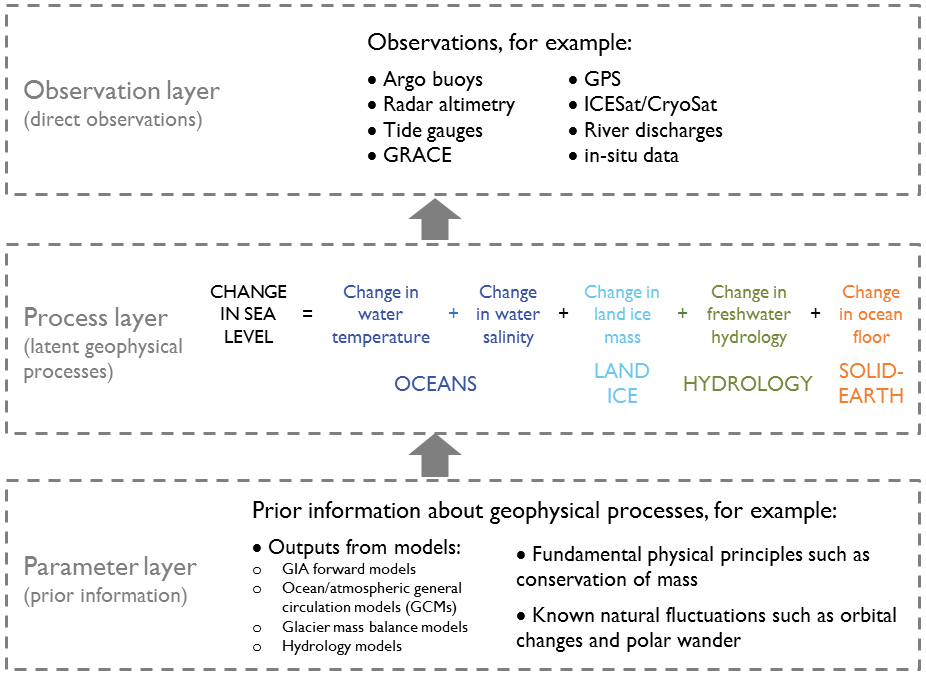
\includegraphics[height = 0.7\textheight]{images/GMconcept-simplified}

\end{frame}

%----------- slide --------------------------------------------------%
\section{modeling the GIA process}
\begin{frame}
\frametitle{What is GIA?}

\end{frame}


%----------- slide --------------------------------------------------%
\begin{frame}{The GIA process}

We assume that the true GIA process is a real-valued spatial process continues on the sphere and denote it by $\bm{Y}: \mathbb{S}^2 \mapsto \mathbb{R}$. We use one of the GIA solution, say from one of the \emph{ice6g} models, as the prior mean of the true process and denote it by $\bm{\mu}: \mathbb{S}^2 \mapsto \mathbb{R}$. Then the residuals between the true process and forward model solutions can be modelled as a stationary Gaussian process on the sphere 
\begin{align}\label{eq:GIAresid}
 \bm{X}: = \bm{Y} - \bm{\mu} \sim \mathcal{GP}(\bm{0}, \kappa(\bm{\theta}))
\end{align}
where $\kappa(\bm{\theta})$ defines the covariance function with hyper parameters $\bm{\theta}$.

\end{frame}

%----------- slide --------------------------------------------------%
\begin{frame}{The GPS data}
The GPS  data are the yearly trends of vertical movements in millimetre at the observed locations. 

In practice, $e_i^2$ can usually be estimated from raw GPS data and therefore we set them to be fixed values from prior information. 
\end{frame}

%----------- slide --------------------------------------------------%
\begin{frame}{From process to observations}
These observations can be regarded as a linear map of the GIA process with measurement errors
\begin{align}\label{eq:GPSi}
Z_i = \bm{\mathcal{A}}_i\bm{Y} + \varepsilon_i, \; i = 1,\dots N.
\end{align} 
where $\bm{\mathcal{A}}_i$ is the linear operator that maps the GIA process to the $i^{\mbox{th}}$ GPS observation and $\varepsilon_i$ are assumed to be independent Gaussian errors $\mathcal{N}(0, e_i^2)$. 

Denote the linear operator for the GPS observation vector $\bm{Z}$ by 
\begin{align*}
\bm{\mathcal{A}} = \left[\begin{array}{c}
 \bm{\mathcal{A}}_1\\ \vdots \\ \bm{\mathcal{A}}_N \end{array} \right]
\end{align*}
Then we can write equation \ref{eq:GPSi} into the vector form
\begin{align}\label{eq:GPS}
\bm{Z} = \bm{\mathcal{A}}\bm{Y} + \bm{\varepsilon} 
\end{align}

\end{frame}

%----------- slide --------------------------------------------------%
\begin{frame}{Bayesian update of the GIA process}
\begin{align}
\left\{ \begin{array}{l}
\bm{\tilde{Z}} = \bm{\mathcal{A}}\bm{X} + \bm{\varepsilon}, \; 
\bm{\varepsilon} \sim \mathcal{N} (\bm{0}, \mbox{diag}(e_1^2, e_2^2, \dots, e_N^2)) \\
\bm{X} \sim \mathcal{GP}(\bm{0}, \kappa(\bm{\theta})) \\
\bm{\theta} \sim \bm{p}(\bm{\theta})
\end{array} \right.
\end{align}
\end{frame}


%----------- Section --------------------------------------------------%
\section{The SPDE Approach}
\begin{frame}{The GMRF approximation}
The Gaussian process model can be computationally expensive for large scale inference since the Bayesian update scales as $\mathcal{O}(m^3)$ mainly due to the inverse of a dense covariance matrix. 

The Gaussian process with Mat\'{e}rn covariance function can be treated as solutions to a class of SPDEs \citep{Lindgren2011} which can then be approximated by GMRF using finite element methods. 

Denote by $\bm{\tilde{X}}$ the GMRF approximation of $\bm{X}$ on a given triangulation of the sphere with piecewise linear basis functions $\{ \bm{\phi}_i \}_{i \in \mathbb{N}}$, then given any location $s \in \mathbb{S}^2$
\begin{align}
\bm{X}(s) \approx \bm{\phi}_i(s)^T\bm{\tilde{X}}
\end{align}
and for a given set $\bm{S}$ of locations, we have  
\begin{align}
\bm{X}(\bm{S}) \approx \bm{C}(\bm{S})\bm{\tilde{X}}
\end{align}
where the matrix $\bm{C}$ contains basis functions for all locations.


\end{frame}

\begin{frame}{The GMRF approximation}
\begin{align}
\left\{ \begin{array}{l}
\bm{\tilde{Z}} = \bm{\mathcal{A}}\bm{C}\bm{\tilde{X}} + \bm{\varepsilon}, \; 
\bm{\varepsilon} \sim \mathcal{N} (\bm{0}, \mbox{diag}(e_1^2, e_2^2, \dots, e_N^2)) \\
\bm{\tilde{X}} \sim \mathcal{N}(\bm{0}, \bm{Q}^{-1}(\bm{\theta})) \\
\bm{\theta} \sim \bm{p}(\bm{\theta})
\end{array} \right.
\end{align}
where $\bm{Q}$ is the precision matrix of the GMRF approximation.

\end{frame}

%----------- slide --------------------------------------------------%
\begin{frame}{Choosing the mesh on sphere}

\end{frame}

%----------- Section --------------------------------------------------%
\section{First result for GIA}
\begin{frame}{First solution for GIA}
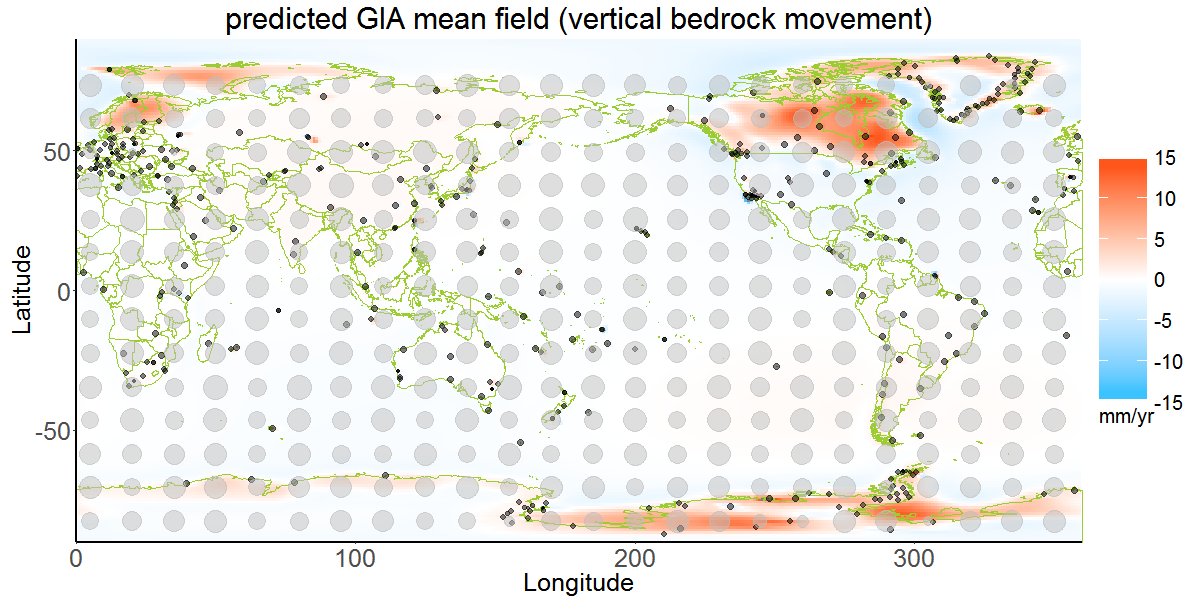
\includegraphics[width = \textwidth]{images/GIA_map}
\end{frame}

%----------- Section --------------------------------------------------%
\section{Conclusion}
\begin{frame}{Conclusion}
Conclusion and future work

\end{frame}


\begin{frame}[plain]
Thank you!
Questions?
\end{frame}


%----------- slide --------------------------------------------------%
\begin{frame}[plain]{References}
\bibliographystyle{plainnat}
\small{\bibliography{references}}
\end{frame}

\end{document}